\documentclass[11pt,a4paper]{report}
\usepackage[textwidth=37em,vmargin=30mm]{geometry}
\usepackage{calc,xunicode,amsmath,amssymb,paralist,enumitem,tabu,booktabs,datetime2,xeCJK,xeCJKfntef,listings}
\usepackage{tocloft,fancyhdr,tcolorbox,xcolor,graphicx,eso-pic,xltxtra,xelatexemoji}

\newcommand{\envyear}[0]{2025}
\newcommand{\envdatestr}[0]{2025-08-08}
\newcommand{\envfinaldir}[0]{webdb/2025/20250808/final}

\usepackage[hidelinks]{hyperref}
\hypersetup{
    colorlinks=false,
    pdfpagemode=FullScreen,
    pdftitle={Web Digest - \envdatestr}
}

\setlength{\cftbeforechapskip}{10pt}
\renewcommand{\cftchapfont}{\rmfamily\bfseries\large\raggedright}
\setlength{\cftbeforesecskip}{2pt}
\renewcommand{\cftsecfont}{\sffamily\small\raggedright}

\setdefaultleftmargin{2em}{2em}{1em}{1em}{1em}{1em}

\usepackage{xeCJK,xeCJKfntef}
\xeCJKsetup{PunctStyle=plain,RubberPunctSkip=false,CJKglue=\strut\hskip 0pt plus 0.1em minus 0.05em,CJKecglue=\strut\hskip 0.22em plus 0.2em}
\XeTeXlinebreaklocale "zh"
\XeTeXlinebreakskip = 0pt


\setmainfont{Brygada 1918}
\setromanfont{Brygada 1918}
\setsansfont{IBM Plex Sans}
\setmonofont{JetBrains Mono NL}
\setCJKmainfont{Noto Serif CJK SC}
\setCJKromanfont{Noto Serif CJK SC}
\setCJKsansfont{Noto Sans CJK SC}
\setCJKmonofont{Noto Sans CJK SC}

\setlength{\parindent}{0pt}
\setlength{\parskip}{8pt}
\linespread{1.15}

\lstset{
	basicstyle=\ttfamily\footnotesize,
	numbersep=5pt,
	backgroundcolor=\color{black!5},
	showspaces=false,
	showstringspaces=false,
	showtabs=false,
	tabsize=2,
	captionpos=b,
	breaklines=true,
	breakatwhitespace=true,
	breakautoindent=true,
	linewidth=\textwidth
}






\newcommand{\coverpic}[2]{
    % argv: itemurl, authorname
    Cover photo by #2~~(\href{#1}{#1})
}
\newcommand{\makeheader}[0]{
    \begin{titlepage}
        % \newgeometry{hmargin=15mm,tmargin=21mm,bmargin=12mm}
        \begin{center}
            
            \rmfamily\scshape
            \fontspec{BaskervilleF}
            \fontspec{Old Standard}
            \fontsize{59pt}{70pt}\selectfont
            WEB\hfill DIGEST
            
            \vfill
            % \vskip 30pt
            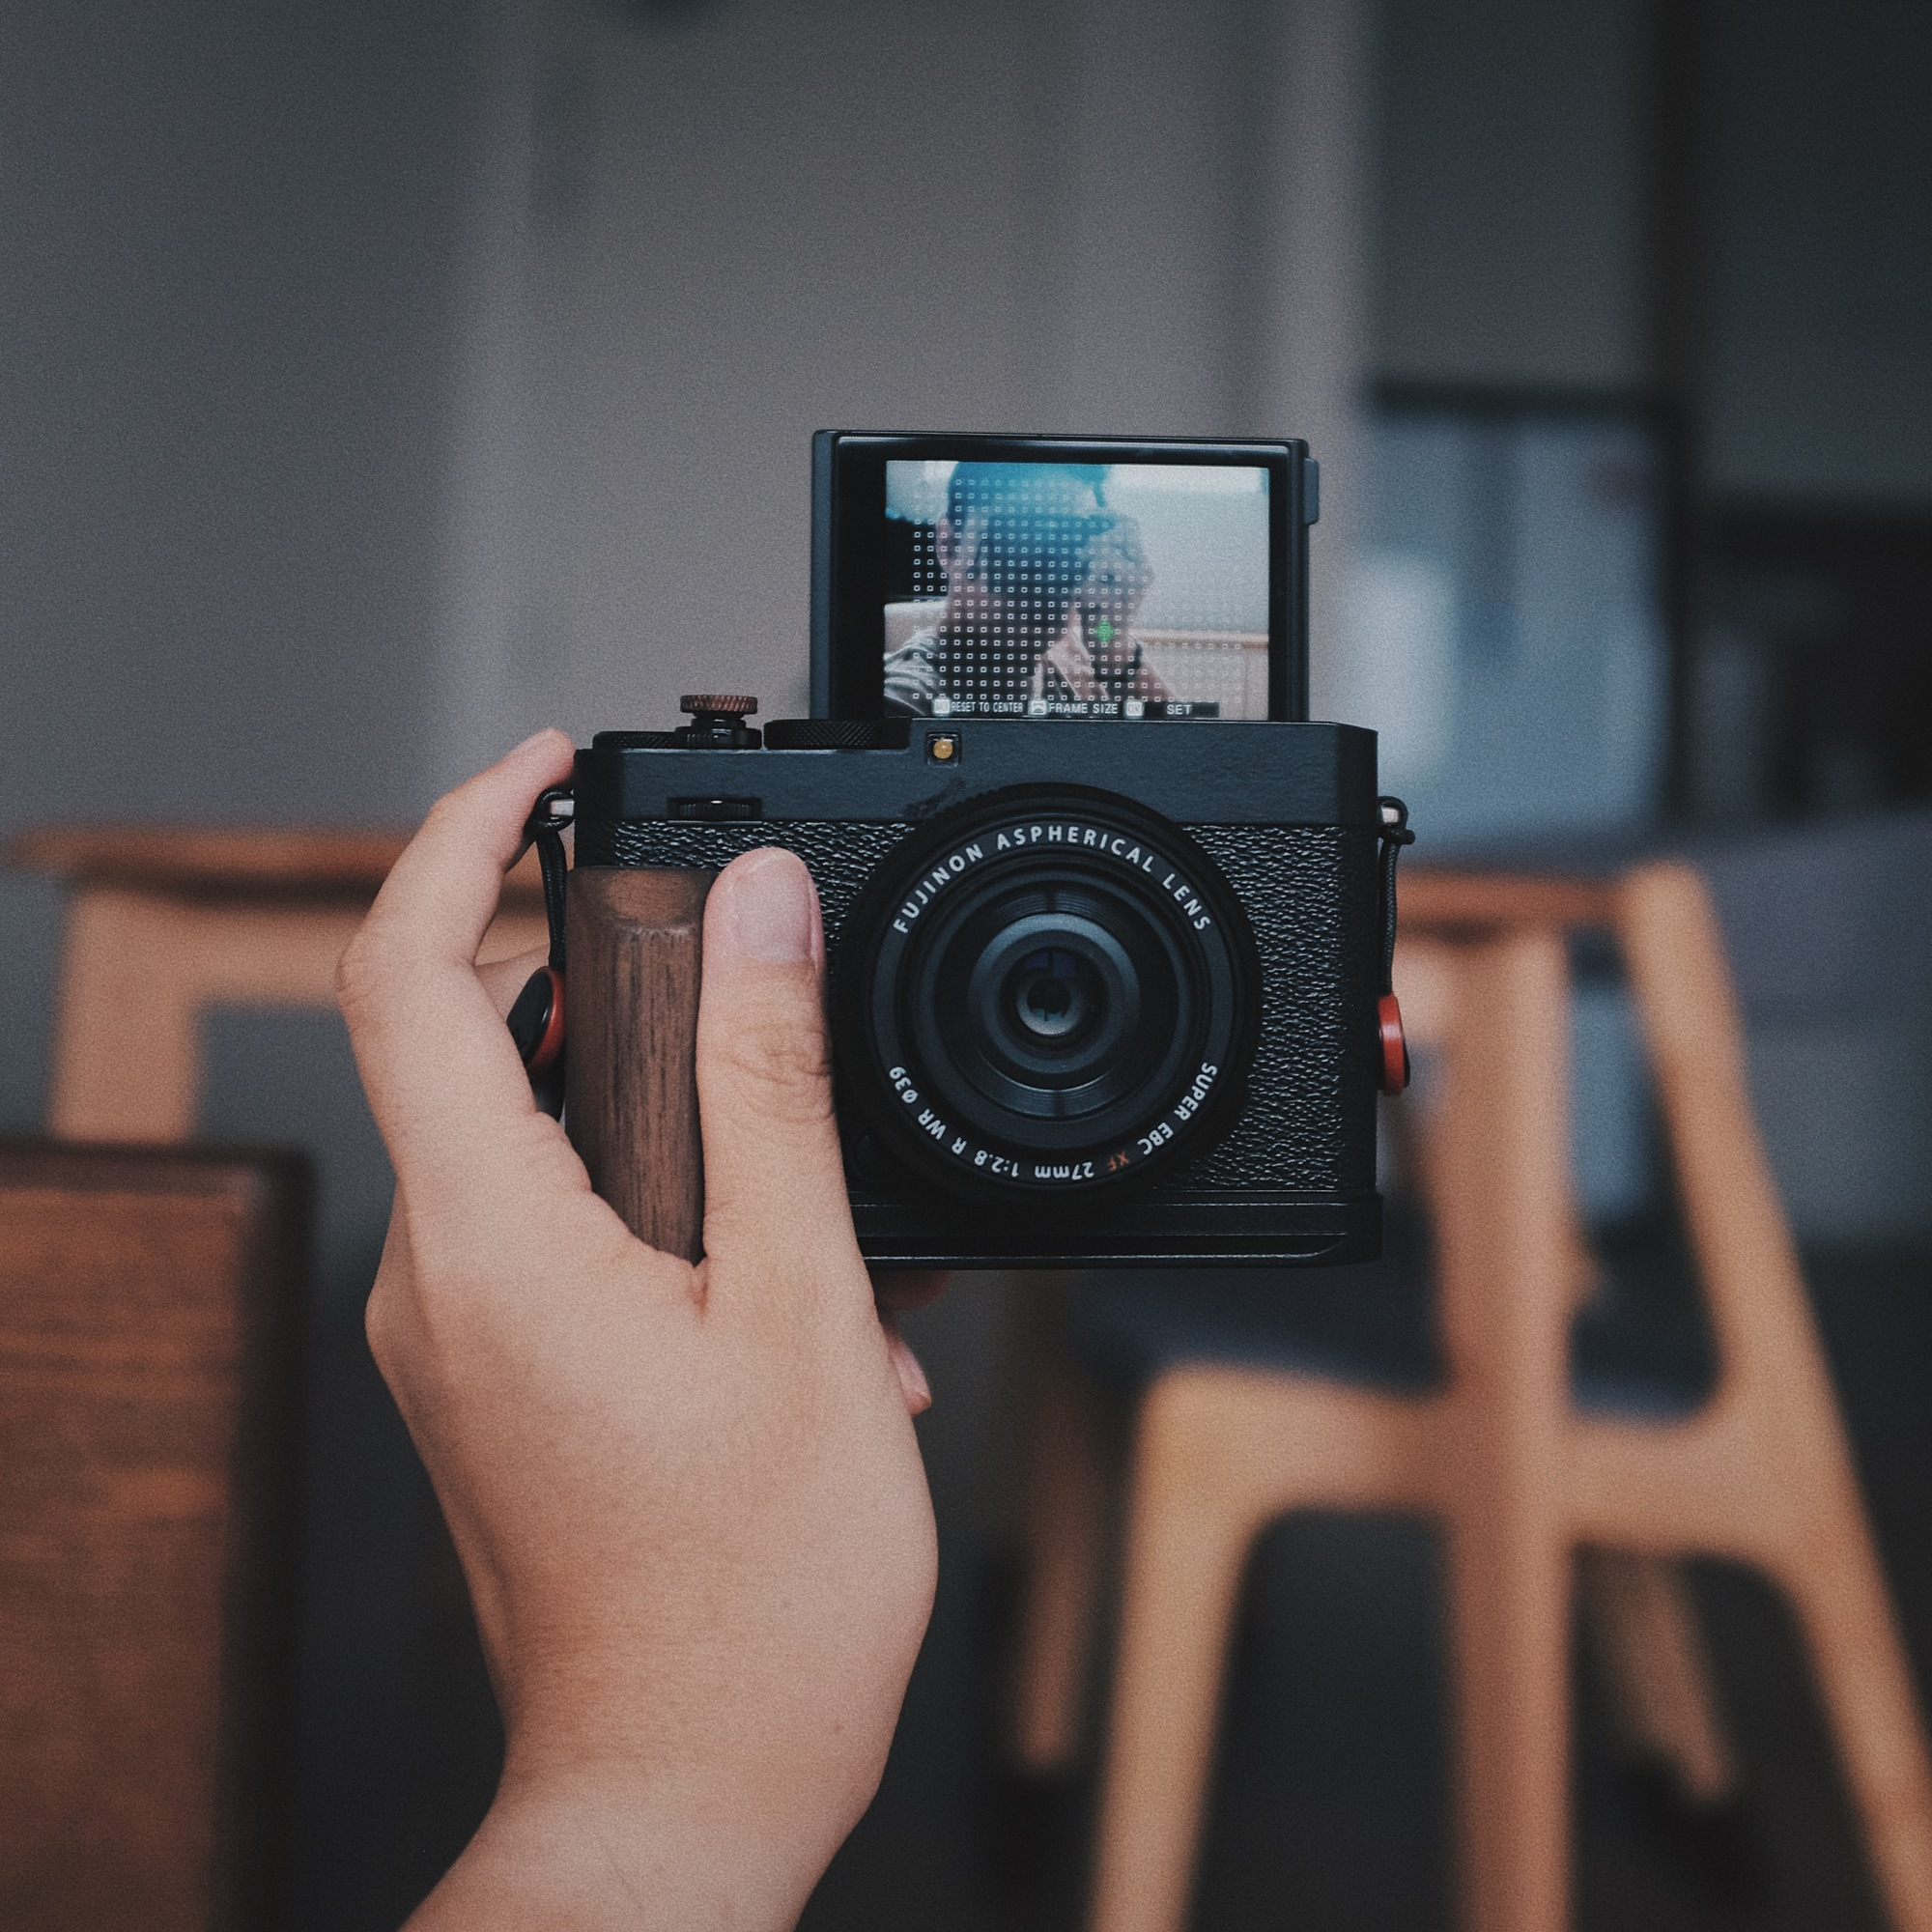
\includegraphics[width=\linewidth]{\envfinaldir/coverpic-prod.jpg}\par
            % \vskip 30pt
            \vfill

            \normalsize\rmfamily\scshape
            \copyright{} The Web Digest Project \hfill\large \envdatestr
        \end{center}
    \end{titlepage}
    % \restoregeometry
}
\newcommand{\simplehref}[1]{%
    \textcolor{blue!80!green}{\href{#1}{#1}}%
}
\renewcommand{\contentsname}{\center\Huge\sffamily\bfseries Contents\par\vskip 20pt}
\newcounter{ipartcounter}
\setcounter{ipartcounter}{0}
\newcommand{\ipart}[1]{
    % \vskip 20pt
    \clearpage
    \stepcounter{ipartcounter}
    \phantomsection
    \addcontentsline{toc}{chapter}{#1}
    % \begin{center}
    %     \Huge
    %     \sffamily\bfseries
    %     #1
    % \end{center}
    % \vskip 20pt plus 7pt
}
\newcounter{ichaptercounter}
\setcounter{ichaptercounter}{0}
\newcommand{\ichapter}[1]{
    % \vskip 20pt
    \clearpage
    \stepcounter{ichaptercounter}
    \phantomsection
    \addcontentsline{toc}{section}{\numberline{\arabic{ichaptercounter}}#1}
    \begin{center}
        \Huge
        \sffamily\bfseries
        #1
    \end{center}
    \vskip 20pt plus 7pt
}
\newcommand{\entrytitlefont}[1]{\subsection*{\raggedright\Large\sffamily\bfseries#1}}
\newcommand{\entryitemGeneric}[2]{
    % argv: title, url
    \parbox{\linewidth}{
        \entrytitlefont{#1}\par\vskip 5pt
        \footnotesize\ttfamily\mdseries
        \simplehref{#2}
    }\vskip 11pt plus 11pt minus 1pt
}
\newcommand{\entryitemGithub}[3]{
    % argv: title, url, desc
    \parbox{\linewidth}{
        \entrytitlefont{#1}\par\vskip 5pt
        \footnotesize\ttfamily\mdseries
        \simplehref{#2}\par\vskip 5pt
        \small\rmfamily\mdseries#3
    }\vskip 11pt plus 11pt minus 1pt
}
\newcommand{\entryitemAp}[3]{
    % argv: title, url, desc
    \parbox{\linewidth}{
        \entrytitlefont{#1}\par\vskip 5pt
        \footnotesize\ttfamily\mdseries
        \simplehref{#2}\par\vskip 5pt
        \small\rmfamily\mdseries#3
    }\vskip 11pt plus 11pt minus 1pt
}
\newcommand{\entryitemHackernews}[3]{
    % argv: title, hnurl, rawurl
    % \parbox{\linewidth}{
    %     \entrytitlefont{#1}\par\vskip 5pt
    %     \footnotesize\ttfamily\mdseries
    %     \simplehref{#3}\par
    %     \textcolor{black!50}{\href{#2}{#2}}
    % }\vskip 11pt plus 11pt minus 1pt
    \begin{minipage}{\linewidth}
            \entrytitlefont{#1}\par\vskip 5pt
            \footnotesize\ttfamily\mdseries
            \simplehref{#3}\par
            \textcolor{black!50}{\href{#2}{#2}}
    \end{minipage}\par\vskip 11pt plus 11pt minus 1pt
}







\begin{document}

\makeheader

\tableofcontents\clearpage




\ipart{Developers}
\ichapter{Hacker News}
\entryitemTwoLinks{Vibechart}{https://news.ycombinator.com/item?id=44830684}{https://www.vibechart.net/}

\entryitemTwoLinks{Cursor CLI}{https://news.ycombinator.com/item?id=44830221}{https://cursor.com/cli}

\entryitemTwoLinks{Historical Tech Tree}{https://news.ycombinator.com/item?id=44829185}{https://www.historicaltechtree.com/}

\entryitemTwoLinks{OpenAI's new open-source model is basically Phi-5}{https://news.ycombinator.com/item?id=44828884}{https://www.seangoedecke.com/gpt-oss-is-phi-5/}

\entryitemTwoLinks{Encryption made for police and military radios may be easily cracked}{https://news.ycombinator.com/item?id=44828504}{https://www.wired.com/story/encryption-made-for-police-and-military-radios-may-be-easily-cracked-researchers-find/}

\entryitemTwoLinks{Benchmark Framework Desktop Mainboard and 4-node cluster}{https://news.ycombinator.com/item?id=44827862}{https://github.com/geerlingguy/ollama-benchmark/issues/21}

\entryitemTwoLinks{GPT-5: Key characteristics, pricing and system card}{https://news.ycombinator.com/item?id=44827794}{https://simonwillison.net/2025/Aug/7/gpt-5/}

\entryitemTwoLinks{GPT-5 for Developers}{https://news.ycombinator.com/item?id=44827101}{https://openai.com/index/introducing-gpt-5-for-developers}

\entryitemTwoLinks{GPT-5}{https://news.ycombinator.com/item?id=44826997}{https://openai.com/gpt-5/}

\entryitemTwoLinks{Live: GPT-5}{https://news.ycombinator.com/item?id=44826463}{https://www.youtube.com/watch?v=0Uu\_VJeVVfo}

\entryitemTwoLinks{Building Bluesky comments for my blog}{https://news.ycombinator.com/item?id=44826164}{https://natalie.sh/posts/bluesky-comments/}

\entryitemTwoLinks{How to sell if your user is not the buyer}{https://news.ycombinator.com/item?id=44825491}{https://writings.founderlabs.io/p/how-to-sell-if-your-user-is-not-the}

\entryitemTwoLinks{Lithium compound can reverse Alzheimer's in mice: study}{https://news.ycombinator.com/item?id=44825326}{https://hms.harvard.edu/news/could-lithium-explain-treat-alzheimers-disease}

\entryitemTwoLinks{Open AI announces \$1.5M bonus for every employee}{https://news.ycombinator.com/item?id=44825309}{https://medium.com/activated-thinker/breaking-open-ai-announces-1-5-million-bonus-for-every-employee-29d057b9d590}

\entryitemTwoLinks{Let's stop pretending that managers and executives care about productivity}{https://news.ycombinator.com/item?id=44824981}{https://www.baldurbjarnason.com/2025/disingenuous-discourse/}

\entryitemTwoLinks{Windows XP Professional}{https://news.ycombinator.com/item?id=44824539}{https://win32.run/}

\entryitemTwoLinks{Infinite Pixels}{https://news.ycombinator.com/item?id=44824056}{https://meyerweb.com/eric/thoughts/2025/08/07/infinite-pixels/}

\entryitemTwoLinks{AI Ethics is being narrowed on purpose, like privacy was}{https://news.ycombinator.com/item?id=44823094}{https://nimishg.substack.com/p/ai-ethics-is-being-narrowed-on-purpose}

\entryitemTwoLinks{The Whispering Earring}{https://news.ycombinator.com/item?id=44822684}{https://croissanthology.com/earring}

\entryitemTwoLinks{How AI conquered the US economy: A visual FAQ}{https://news.ycombinator.com/item?id=44822665}{https://www.derekthompson.org/p/how-ai-conquered-the-us-economy-a}\ichapter{Phoronix}
\entryitemGeneric{\hskip 0pt{}New AMD Zen 6 Linux Patches Posted - Confirming Up To 16 Memory Channels}{https://www.phoronix.com/news/AMD-Zen-6-Venice-16c-RAM}

\entryitemGeneric{\hskip 0pt{}Linux 6.17 Standardizes The Keycode For The "Performance Boost" Key}{https://www.phoronix.com/news/Linux-6.17-Performance-Key}

\entryitemGeneric{\hskip 0pt{}Redox OS Recently Saw 500~700\% Performance Improvement For Basic File I/O}{https://www.phoronix.com/news/Redox-OS-July-2025}

\entryitemGeneric{\hskip 0pt{}AMD Ryzen AI Max+ 395 vs. Ryzen 9 9950X vs. Ryzen 9 9950X3D Linux Performance}{https://www.phoronix.com/review/ryzen-ai-max-395-9950x-9950x3d}

\entryitemGeneric{\hskip 0pt{}Framework Desktop With AMD Ryzen AI Max Offers Excellent, Linux-Friendly Performance}{https://www.phoronix.com/review/framework-desktop-linux}

\entryitemGeneric{\hskip 0pt{}Ubuntu 24.04.3 LTS Released With Linux 6.14 HWE Kernel}{https://www.phoronix.com/news/Ubuntu-24.04.3-LTS-Released}

\entryitemGeneric{\hskip 0pt{}Heterogeneous CPU Cores, HDMI \& Other Work Continues For Enhancing FreeBSD On Laptops}{https://www.phoronix.com/news/FreeBSD-Laptops-July-2025}

\entryitemGeneric{\hskip 0pt{}Rust 1.89 Released With More AVX-512 Intrinsics \& x86 Target Features}{https://www.phoronix.com/news/Rust-1.89-Released}

\entryitemGeneric{\hskip 0pt{}Flang-Tidy Cleaning/Correcting Fortran Code In "Sort Of Opinionated Fashion"}{https://www.phoronix.com/news/Flang-Tidy}


\ipart{Developers~~~~(zh-Hans)}
\ichapter{Solidot}
\entryitemGeneric{\hskip 0pt{}特朗普威胁对芯片征收 100\% 关税,除非在美建厂或承诺建厂}{https://www.solidot.org/story?sid=81983}

\entryitemGeneric{\hskip 0pt{}日本禁止苹果 iOS 限制第三方浏览器引擎}{https://www.solidot.org/story?sid=81982}

\entryitemGeneric{\hskip 0pt{}Grok 未经用户要求就生成斯威夫特的裸照}{https://www.solidot.org/story?sid=81981}

\entryitemGeneric{\hskip 0pt{}维基百科编辑对 AI 生成文章采用加速删除政策}{https://www.solidot.org/story?sid=81980}

\entryitemGeneric{\hskip 0pt{}GitHub CEO 警告开发者要么拥抱 AI 要么改行}{https://www.solidot.org/story?sid=81979}

\entryitemGeneric{\hskip 0pt{}Proxmox Virtual Environment 9.0 释出}{https://www.solidot.org/story?sid=81978}

\entryitemGeneric{\hskip 0pt{}瑞典首相因在工作中使用 AI 工具而受到批评}{https://www.solidot.org/story?sid=81977}

\entryitemGeneric{\hskip 0pt{}OpenAI 自 GPT-2 以来首次发布开放权重模型}{https://www.solidot.org/story?sid=81976}

\entryitemGeneric{\hskip 0pt{}美科技企业今年前七个月裁员 9 万人}{https://www.solidot.org/story?sid=81975}

\entryitemGeneric{\hskip 0pt{}英伟达否认其产品含有后门和关闭开关}{https://www.solidot.org/story?sid=81974}

\entryitemGeneric{\hskip 0pt{}台积电指控前雇员窃取 2 纳米芯片技术机密}{https://www.solidot.org/story?sid=81973}

\entryitemGeneric{\hskip 0pt{}科学家研发出一种效力与吗啡相当但无严重副作用的止痛药}{https://www.solidot.org/story?sid=81972}

\entryitemGeneric{\hskip 0pt{}用激光穿透人类大脑}{https://www.solidot.org/story?sid=81971}

\entryitemGeneric{\hskip 0pt{}超加工饮食减肥的效果不大}{https://www.solidot.org/story?sid=81970}

\entryitemGeneric{\hskip 0pt{}特斯拉被指在涉及自动驾驶的车祸案件中隐瞒数据、撒谎和误导警方}{https://www.solidot.org/story?sid=81969}

\entryitemGeneric{\hskip 0pt{}大型流浪行星可能会形成自己的微型行星系统}{https://www.solidot.org/story?sid=81968}

\entryitemGeneric{\hskip 0pt{}Perplexity 使用隐蔽策略绕过网站禁止抓取的指令}{https://www.solidot.org/story?sid=81967}

\entryitemGeneric{\hskip 0pt{}乌克兰通过无人机快递电动自行车救出士兵}{https://www.solidot.org/story?sid=81966}\ichapter{V2EX}
\entryitemGeneric{\hskip 0pt{}[问与答] 有 V 友看过现实中的 F1 赛车吗,我今天坐动车在站台等候时候(我排在第一个),一辆不停站动车从我面前开过,瞬间肾上腺素飙升。F1 是不是也是这种感觉}{https://www.v2ex.com/t/1150871}

\entryitemGeneric{\hskip 0pt{}[问与答] PD 快充给小家电充电必须自己 diy 么?}{https://www.v2ex.com/t/1150870}

\entryitemGeneric{\hskip 0pt{}[Solana] 20250807 - 打赏按钮已经添加到手机版网页}{https://www.v2ex.com/t/1150869}

\entryitemGeneric{\hskip 0pt{}[问与答] 求推荐个 32 4K 的显示器? 办公用 不需要太好 预算 2k 杂牌都可以}{https://www.v2ex.com/t/1150867}

\entryitemGeneric{\hskip 0pt{}[Linux] 6.16 内核 桌面用户还是值得升级的}{https://www.v2ex.com/t/1150866}

\entryitemGeneric{\hskip 0pt{}[OpenAI] ChatGPT 5 上了}{https://www.v2ex.com/t/1150865}

\entryitemGeneric{\hskip 0pt{}[macOS] Mac beta 先不要升到 beta5 聚焦内存可能有泄漏}{https://www.v2ex.com/t/1150863}

\entryitemGeneric{\hskip 0pt{}[分享发现] 分享个大厂提供的获取当前 IP 信息的接口,稳定可靠,适合硬编码进脚本}{https://www.v2ex.com/t/1150862}

\entryitemGeneric{\hskip 0pt{}[macOS] macOS 26 public beta2 更新了}{https://www.v2ex.com/t/1150861}

\entryitemGeneric{\hskip 0pt{}[OpenAI] ChatGPT 5 来了,各位怎么看?}{https://www.v2ex.com/t/1150860}

\entryitemGeneric{\hskip 0pt{}[分享创造] 开发了一个简单的音域检测工具}{https://www.v2ex.com/t/1150859}

\entryitemGeneric{\hskip 0pt{}[Solana] 发现\$V2EX 半夜有人套现 80+k,把价格打下来了, DEV 及时买入}{https://www.v2ex.com/t/1150858}

\entryitemGeneric{\hskip 0pt{}[程序员] 淘宝开发来领 bug 了:才半年,淘宝账户就第二次被错误封控}{https://www.v2ex.com/t/1150857}

\entryitemGeneric{\hskip 0pt{}[海外留学] 关于赴美读研/签证受阻/未来选择的极度焦虑,想听听大家的建议}{https://www.v2ex.com/t/1150855}

\entryitemGeneric{\hskip 0pt{}[职场话题] 感觉经济实在是不太好,北美的朋友聊一聊?}{https://www.v2ex.com/t/1150853}

\entryitemGeneric{\hskip 0pt{}[Go 编程语言] golang 在 Windows 下,网络 io 资源消耗似乎比比 Linux 高一些}{https://www.v2ex.com/t/1150852}

\entryitemGeneric{\hskip 0pt{}[Solana] web3 水太深,买到一个假币,被抽干流动性,卖不掉了}{https://www.v2ex.com/t/1150851}

\entryitemGeneric{\hskip 0pt{}[Solana] 为什么 V2EX 市值这么高?}{https://www.v2ex.com/t/1150850}

\entryitemGeneric{\hskip 0pt{}[程序员] Gemini 写论文非常好用}{https://www.v2ex.com/t/1150849}

\entryitemGeneric{\hskip 0pt{}[路由器] 有人遇到多线路下 ros7 自带 wg 服务回流错误的问题吗?}{https://www.v2ex.com/t/1150848}

\entryitemGeneric{\hskip 0pt{}[问与答] 求助 windows 经常弹出 程序兼容性助手 此模块被阻止加载到本地安全机构}{https://www.v2ex.com/t/1150847}

\entryitemGeneric{\hskip 0pt{}[职场话题] 大厂被裁,躺平 2 年后如何快速重新开始}{https://www.v2ex.com/t/1150844}

\entryitemGeneric{\hskip 0pt{}[全球工单系统] 钉钉 Linux 客户端能够下载群中保密视频的 bug}{https://www.v2ex.com/t/1150843}

\entryitemGeneric{\hskip 0pt{}[PRO] 功能建议:主题回复权限设置}{https://www.v2ex.com/t/1150840}

\entryitemGeneric{\hskip 0pt{}[旅行] 很多景点,只看照片是没法亲身体会现场的}{https://www.v2ex.com/t/1150838}

\entryitemGeneric{\hskip 0pt{}[互联网] 一打开高德, AI 深度思考我要去哪,推荐导航到 3 个月没去过的地方}{https://www.v2ex.com/t/1150837}

\entryitemGeneric{\hskip 0pt{}[程序员] 🚀 iOS 开发神器:一键打包 XCFramework,告别手动构建烦恼}{https://www.v2ex.com/t/1150836}

\entryitemGeneric{\hskip 0pt{}[武汉] 武汉有没有老饭馆,求推荐}{https://www.v2ex.com/t/1150834}

\entryitemGeneric{\hskip 0pt{}[旅行] 大佬们一个人去日本想玩儿 7 天的话, 1 万够么?签证好办么?}{https://www.v2ex.com/t/1150833}

\entryitemGeneric{\hskip 0pt{}[智能家电] 怎么才能比较容易的每个房间放一个音箱?}{https://www.v2ex.com/t/1150832}

\entryitemGeneric{\hskip 0pt{}[远程工作] 量化 / LLM 算法 / 全栈}{https://www.v2ex.com/t/1150831}

\entryitemGeneric{\hskip 0pt{}[宽带症候群] 自建 NetBird 稳定吗?}{https://www.v2ex.com/t/1150830}

\entryitemGeneric{\hskip 0pt{}[问与答] 有没有能正常浏览网页的代理 IP 池推荐?}{https://www.v2ex.com/t/1150829}

\entryitemGeneric{\hskip 0pt{}[随想] 想请问大家今年压力大吗?}{https://www.v2ex.com/t/1150828}

\entryitemGeneric{\hskip 0pt{}[分享发现] 收到了 10 年前给自己写的信}{https://www.v2ex.com/t/1150827}

\entryitemGeneric{\hskip 0pt{}[Solana] 空置的钱包可以使用这个网站来回收, 每个能回收 0.002sol}{https://www.v2ex.com/t/1150825}

\entryitemGeneric{\hskip 0pt{}[Google] Gemini CLI 号称的每天 1000 万 tokens 和 1000 次请求}{https://www.v2ex.com/t/1150824}

\entryitemGeneric{\hskip 0pt{}[阅读] 问一个小说的名字,印象中是在 2010 年左右看到的网文}{https://www.v2ex.com/t/1150823}

\entryitemGeneric{\hskip 0pt{}[Solana] 大家注意 Solana 链上有个 V2EX 山寨币}{https://www.v2ex.com/t/1150822}

\entryitemGeneric{\hskip 0pt{}[问与答] 电脑组装求助}{https://www.v2ex.com/t/1150821}

\entryitemGeneric{\hskip 0pt{}[分享创造] [小程序]开发了一个老照片修复小帮手,基于 Kontext}{https://www.v2ex.com/t/1150820}

\entryitemGeneric{\hskip 0pt{}[Solana] 最近 V2EX 赚了,开一轮打赏,请各位没有收到过打赏的留言,打赏前 50 名}{https://www.v2ex.com/t/1150819}

\entryitemGeneric{\hskip 0pt{}[分享创造] 写了一个在线 epub 合并工具网站,有需要的自取}{https://www.v2ex.com/t/1150818}

\entryitemGeneric{\hskip 0pt{}[.NET] [分享创造] 开源轻量级 WinForm 壁纸切换器 Wallpaper Switcher (C\# / .NET 9)}{https://www.v2ex.com/t/1150815}

\entryitemGeneric{\hskip 0pt{}[Solana] v2ex.fun 能做点啥?专门做个和\$v2ex 有关的站点?}{https://www.v2ex.com/t/1150814}

\entryitemGeneric{\hskip 0pt{}[iOS] iOS 上的米家自动化替代方案:用快捷指令 + 中转服务实现设备控制}{https://www.v2ex.com/t/1150813}

\entryitemGeneric{\hskip 0pt{}[Solana] 币安的通行密钥(生物识别)一直添加失败}{https://www.v2ex.com/t/1150812}

\entryitemGeneric{\hskip 0pt{}[优惠信息] 饿了么 19-18,限时的,速度}{https://www.v2ex.com/t/1150810}

\entryitemGeneric{\hskip 0pt{}[生活] 家里人在拼多多给小孩买的零食掺着老鼠药,能索赔吗}{https://www.v2ex.com/t/1150809}

\entryitemGeneric{\hskip 0pt{}[酷工作] [内推] [深圳] [大疆创新] [前端开发、后端开发、产品经理、GIS 开发、 算法工程师(三维重建)]}{https://www.v2ex.com/t/1150808}


\ipart{Generic News}







\clearpage
\leavevmode\vfill
\footnotesize

Copyright \copyright{} 2023-2025 Neruthes and other contributors.

This document is published with CC BY-NC-ND 4.0 license.

The entries listed in this newsletter may be copyrighted by their respective creators.

This newsletter is generated by the Web Digest project.

The newsletters are also delivered via Telegram channel \CJKunderline{\href{https://t.me/webdigestchannel}{https://t.me/webdigestchannel}}.\\
RSS feed is available at \CJKunderline{\href{https://webdigest.pages.dev/rss.xml}{https://webdigest.pages.dev/rss.xml}}.

This newsletter is available in PDF at
\CJKunderline{\href{https://webdigest.pages.dev/}{https://webdigest.pages.dev/}}.

The source code being used to generate this newsletter is available at\\
\CJKunderline{\href{https://github.com/neruthes/webdigest}{https://github.com/neruthes/webdigest}}.

This newsletter is also available in
\CJKunderline{\href{http://webdigest.pages.dev/readhtml/\envyear/WebDigest-20250808.html}{HTML}} and
\CJKunderline{\href{https://github.com/neruthes/webdigest/blob/master/markdown/\envyear/WebDigest-20250808.md}{Markdown}}.


\coverpic{https://unsplash.com/photos/stone-arches-stand-in-a-foggy-landscape-amGbJl\_s1hU}{Joseph Corl}


\end{document}
